\documentclass[tikz]{standalone}
\usepackage{amssymb,amsmath,mathtools}

\usetikzlibrary{fit}
\usetikzlibrary{shapes,arrows}
\usetikzlibrary {shapes.misc} 
\usetikzlibrary{arrows.meta}
\usetikzlibrary{calc,positioning}
\usetikzlibrary{patterns,decorations.pathmorphing,decorations.markings}

\begin{document}

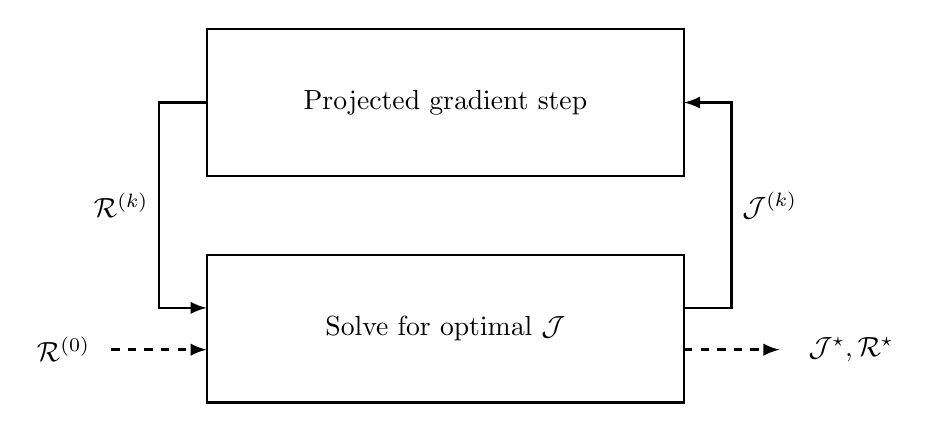
\begin{tikzpicture}
    \tikzstyle{dashed line} = [draw, dashed, line width=1pt, -latex]
    \tikzstyle{line} = [draw, very thick, line width=1pt, -latex]

    \def\blockWidth{0.5\linewidth}
    \def\blockHeight{0.5 * \blockWidth*0.61803399}

    \node[draw,outer sep=0pt,thick] (B1) [minimum width=\blockWidth, minimum height=\blockHeight] {Projected gradient step};

    \node[draw,outer sep=0pt,thick] (B2) [minimum width=\blockWidth, minimum height=\blockHeight, below of=B1, yshift=-\blockHeight] {Solve for optimal $\mathcal{J}$};
    
    \node (input) [%
        coordinate,
        xshift=-0.2*\blockWidth,
    ] at (B2.185) {};

    \node (output) [%
        coordinate,
        xshift=0.2*\blockWidth,
    ] at (B2.355) {};

    \node (iB1) [%
        align=center,
        xshift=0.6*\blockWidth,
        coordinate
    ] at (B1) {};

    \node (B1o) [%
        align=center,
        xshift=-0.6*\blockWidth,
        coordinate
    ] at (B1) {};
    
    \node (B2o) [%
        align=center,
        xshift=0.1*\blockWidth,
        coordinate
    ] at (B2.5) {};
    
    \path [dashed line] (input) -- (B2.185);
    \path [dashed line] (B2.355) -- (output);

    \node (R0) [
        align=center,
        xshift=-0.1*\blockWidth,
    ] at (input) {$\mathcal{R}^{(0)}$};

    \node (minimizer) [
        align=center,
        xshift=0.15*\blockWidth,
    ] at (output) {$\mathcal{J}^\star,\mathcal{R}^\star$};

    \path [line] (B2.5) -- (B2o) |- (B1) node [right, pos=0.25] {$\mathcal{J}^{(k)}$};
    \path [line] (B1) --  (B1o) |-  (B2.175) node [left, pos=0.25] {$\mathcal{R}^{(k)}$};
        \end{tikzpicture}

\end{document}